\section{Системийн шаардлага}

Функциональ шаардлага нь системийн гол үйл ажиллагааг тодорхойлж, хэрэглэгчдэд ямар боломж олгохыг заана.
Эдгээр шаардлагууд нь системийн үндсэн зорилтыг хангахад чиглэсэн бөгөөд хэрэглэгчийн туршлагыг сайжруулах,
гүйцэтгэлийн үнэлгээний процессийг автоматжуулахад тусална. Шаардлагуудыг ерөнхий шаардлага болон хэрэглэгчийн
төрлүүдээр (Админ, Менежер (хүний нөөцийн мэргэжилтэн), Ажилтан) ангилан доорх хүснэгтүүдэд дэлгэрэнгүй харуулав.

\subsection{Функциональ шаардлага}
\subsubsection{Ерөнхий шаардлага}
Ерөнхий шаардлагууд нь системийн суурь үйл ажиллагааг хамардаг бөгөөд бүх хэрэглэгчидтэй холбоотой үндсэн 
функцуудыг тодорхойлно. Эдгээр нь системийн аюулгүй байдал, хэрэглэгчийн бүртгэл, мэдээлэл хандалт зэрэгт чиглэнэ.

\begin{table}[H]
    \centering
    \label{my-label-1}
    \begin{tabular}{|p{1.7cm}|p{12cm}|}
        \hline
          ФШ100 & Хэрэглэгч бүртгэдэг байх\\\hline
          ФШ101 & Хэрэглэгчийн хувийн мэдээлэл харуулдаг байх\\ \hline
          ФШ102 & Хэрэглэгчийн оролцсон төсөл, даалгавар харуулдаг байх \\\hline
          ФШ103 & Даалгавар үүсгэх \\ \hline
          ФШ104 & Системийн лог хөтлөдөг байх\\ \hline
          ФШ105 & Хэрэглэгчийн session удирддаг байх \\ \hline
    \end{tabular}
    \caption{Ерөнхий шаардлага}
\end{table}

\subsubsection{Админ шаардлага}
Системийн удирдлага, аюулгүй байдал, засвар үйлчилгээтэй холбоотой бөгөөд системийн тогтвортой байдлыг хангахад чиглэнэ.

\begin{table}[H]
    \centering
    \label{my-label-2}
    \begin{tabular}{|p{1.7cm}|p{12cm}|}
        \hline
          АФШ200 & Хэрэглэгчийн эрхийг удирддаг байх\\ \hline
          АФШ201 & Системийн тохиргоог өөрчилдөг байх\\ \hline
          АФШ202 & Мэдээллийн сангийн нөөцлөлт, сэргээлт хийдэг байх\\\hline
          АФШ203 & Бүх хэрэглэгчийн үйлдлийн түүхийг хянах\\ \hline
    \end{tabular}
    \caption{Админ шаардлага}
\end{table}

\subsubsection{Менежер шаардлага}
Ажилтны гүйцэтгэлийг удирдах, хянах, тайлагнахад чиглэсэн бөгөөд системийн гол зорилгыг хэрэгжүүлэхэд тусална.

\begin{table}[H]
    \centering
    \label{my-label-3}
    \begin{tabular}{|p{1.7cm}|p{12cm}|}
        \hline
          МФШ300 & Даалгавар үүсгэж, хуваарилдаг байх\\ \hline
          МФШ301 & Даалгаврын гүйцэтгэлийн явцыг хянадаг байх\\ \hline
          МФШ302 & Ажилтны гүйцэтгэлийг KPI-д суурилан үнэлгээг автоматаар гаргадаг байх\\\hline
          МФШ303 & Тайлан гаргадаг байх\\ \hline
          МФШ304 & Тайланг PDF эсвэл CSV татаж авах боломжтой байх\\ \hline
    \end{tabular}
    \caption{Менежер шаардлага}
\end{table}

\subsubsection{Ажилтан шаардлага}
Хувь хүний гүйцэтгэлийг хянах, даалгавар удирдахад чиглэсэн бөгөөд хэрэглэгчийн идэвхийг дэмжинэ.

\begin{table}[H]
    \centering
    \label{my-label-4}
    \begin{tabular}{|p{1.7cm}|p{12cm}|}
        \hline
        АФШ400 & Даалгавар үүсгэдэг байх\\ \hline
        АФШ401 & Даалгаврын үйл явцыг удирдах\\ \hline
        АФШ402 & Өөртөө үнэлгээ өгөх\\\hline
        АФШ403 & Өөрийн үнэлгээг хянах\\ \hline
    \end{tabular}
    \caption{Ажилтан шаардлага}
\end{table}

\subsection{Функциональ биш шаардлага}

\begin{table}[H]
    \centering
    \label{my-label-5}
    \begin{tabular}{|p{1.7cm}|p{12cm}|}
        \hline
        ФБШ100 & Систем нь 24/7 ажиллах чадвартай байх\\ \hline
        ФБШ101 & Систем нь веб сайтын стандартыг дагаж мөрдөх\\ \hline
        ФБШ102 & Систем нь аюулгүй байдал сайтай байх\\ \hline
        ФБШ103 & Хэрэглэгчийн нэвтрэх мэдээллийг хамгаалдаг байх\\ \hline
        ФБШ104 & Хэрэглэгчийн нууц үгийг шифрлэдэг байх\\ \hline
        ФБШ105 & Системийн хариулах хугацаа 3 секундээс бага байх\\ \hline
        ФБШ106 & Хэрэглэгчийн хандалтад хязгаарлалт тавих\\ \hline
    \end{tabular}
    \caption{Функциональ биш шаардлага}
\end{table}

\subsection{Системийн шаардлага}

\begin{table}[H]
    \centering
    \label{my-label-6}
    \begin{tabular}{|p{1.7cm}|p{12cm}|}
        \hline
        СШ500 & Систем нь өгөгдлийн санг үр дүнтэй удирдаж, мэдээллийг хадгалах,
        устгах, шинэчлэх функцуудтай байх\\ \hline
        СШ501 & Систем нь хэрэглэгчийн эрхүүдийг хянаж, админ, ажилтан зэрэг
        түвшингийн хэрэглэгчдэд тохирсон эрх олгох\\ \hline
        СШ502 & Эрхээс шалтгаалж харагдац өөр байх\\ \hline
        СШ503 & Хэрэглэгчийн нэвтрэх мэдээллийг хамгаалдаг байх\\ \hline
        СШ504 & Хэрэглэгчийн нууц үгийг шифрлэдэг байх\\ \hline
    \end{tabular}
    \caption{Функциональ биш шаардлага}
\end{table}

\subsection{UI/UX шаардлага}
Уг системийн гол үйл ажилгаа гүйцэтгэлийн үнэлгээг ихэвчлэн суурин компьютер дээр гаргах учир админ болон
менежерийн харагдац үүнд тохирсон байх. Харин ажилтны хувьд гар утаснаас хандах боломжыг нэмж өгөх хэрэгтэй.
Суурь вебд апп нь динамик хариу үйлдэл үзүүлдэг тул үүн дээр асуудал гарахгүй.

\subsubsection{Нэвтрэх хуудас}
Системийн нэвтрэх хэсэг хэрэглэгчийн хандах эрхээс үл шалтгаалж нэгэн адил харагдацтай байна.
\begin{figure}[h]
    \centering
    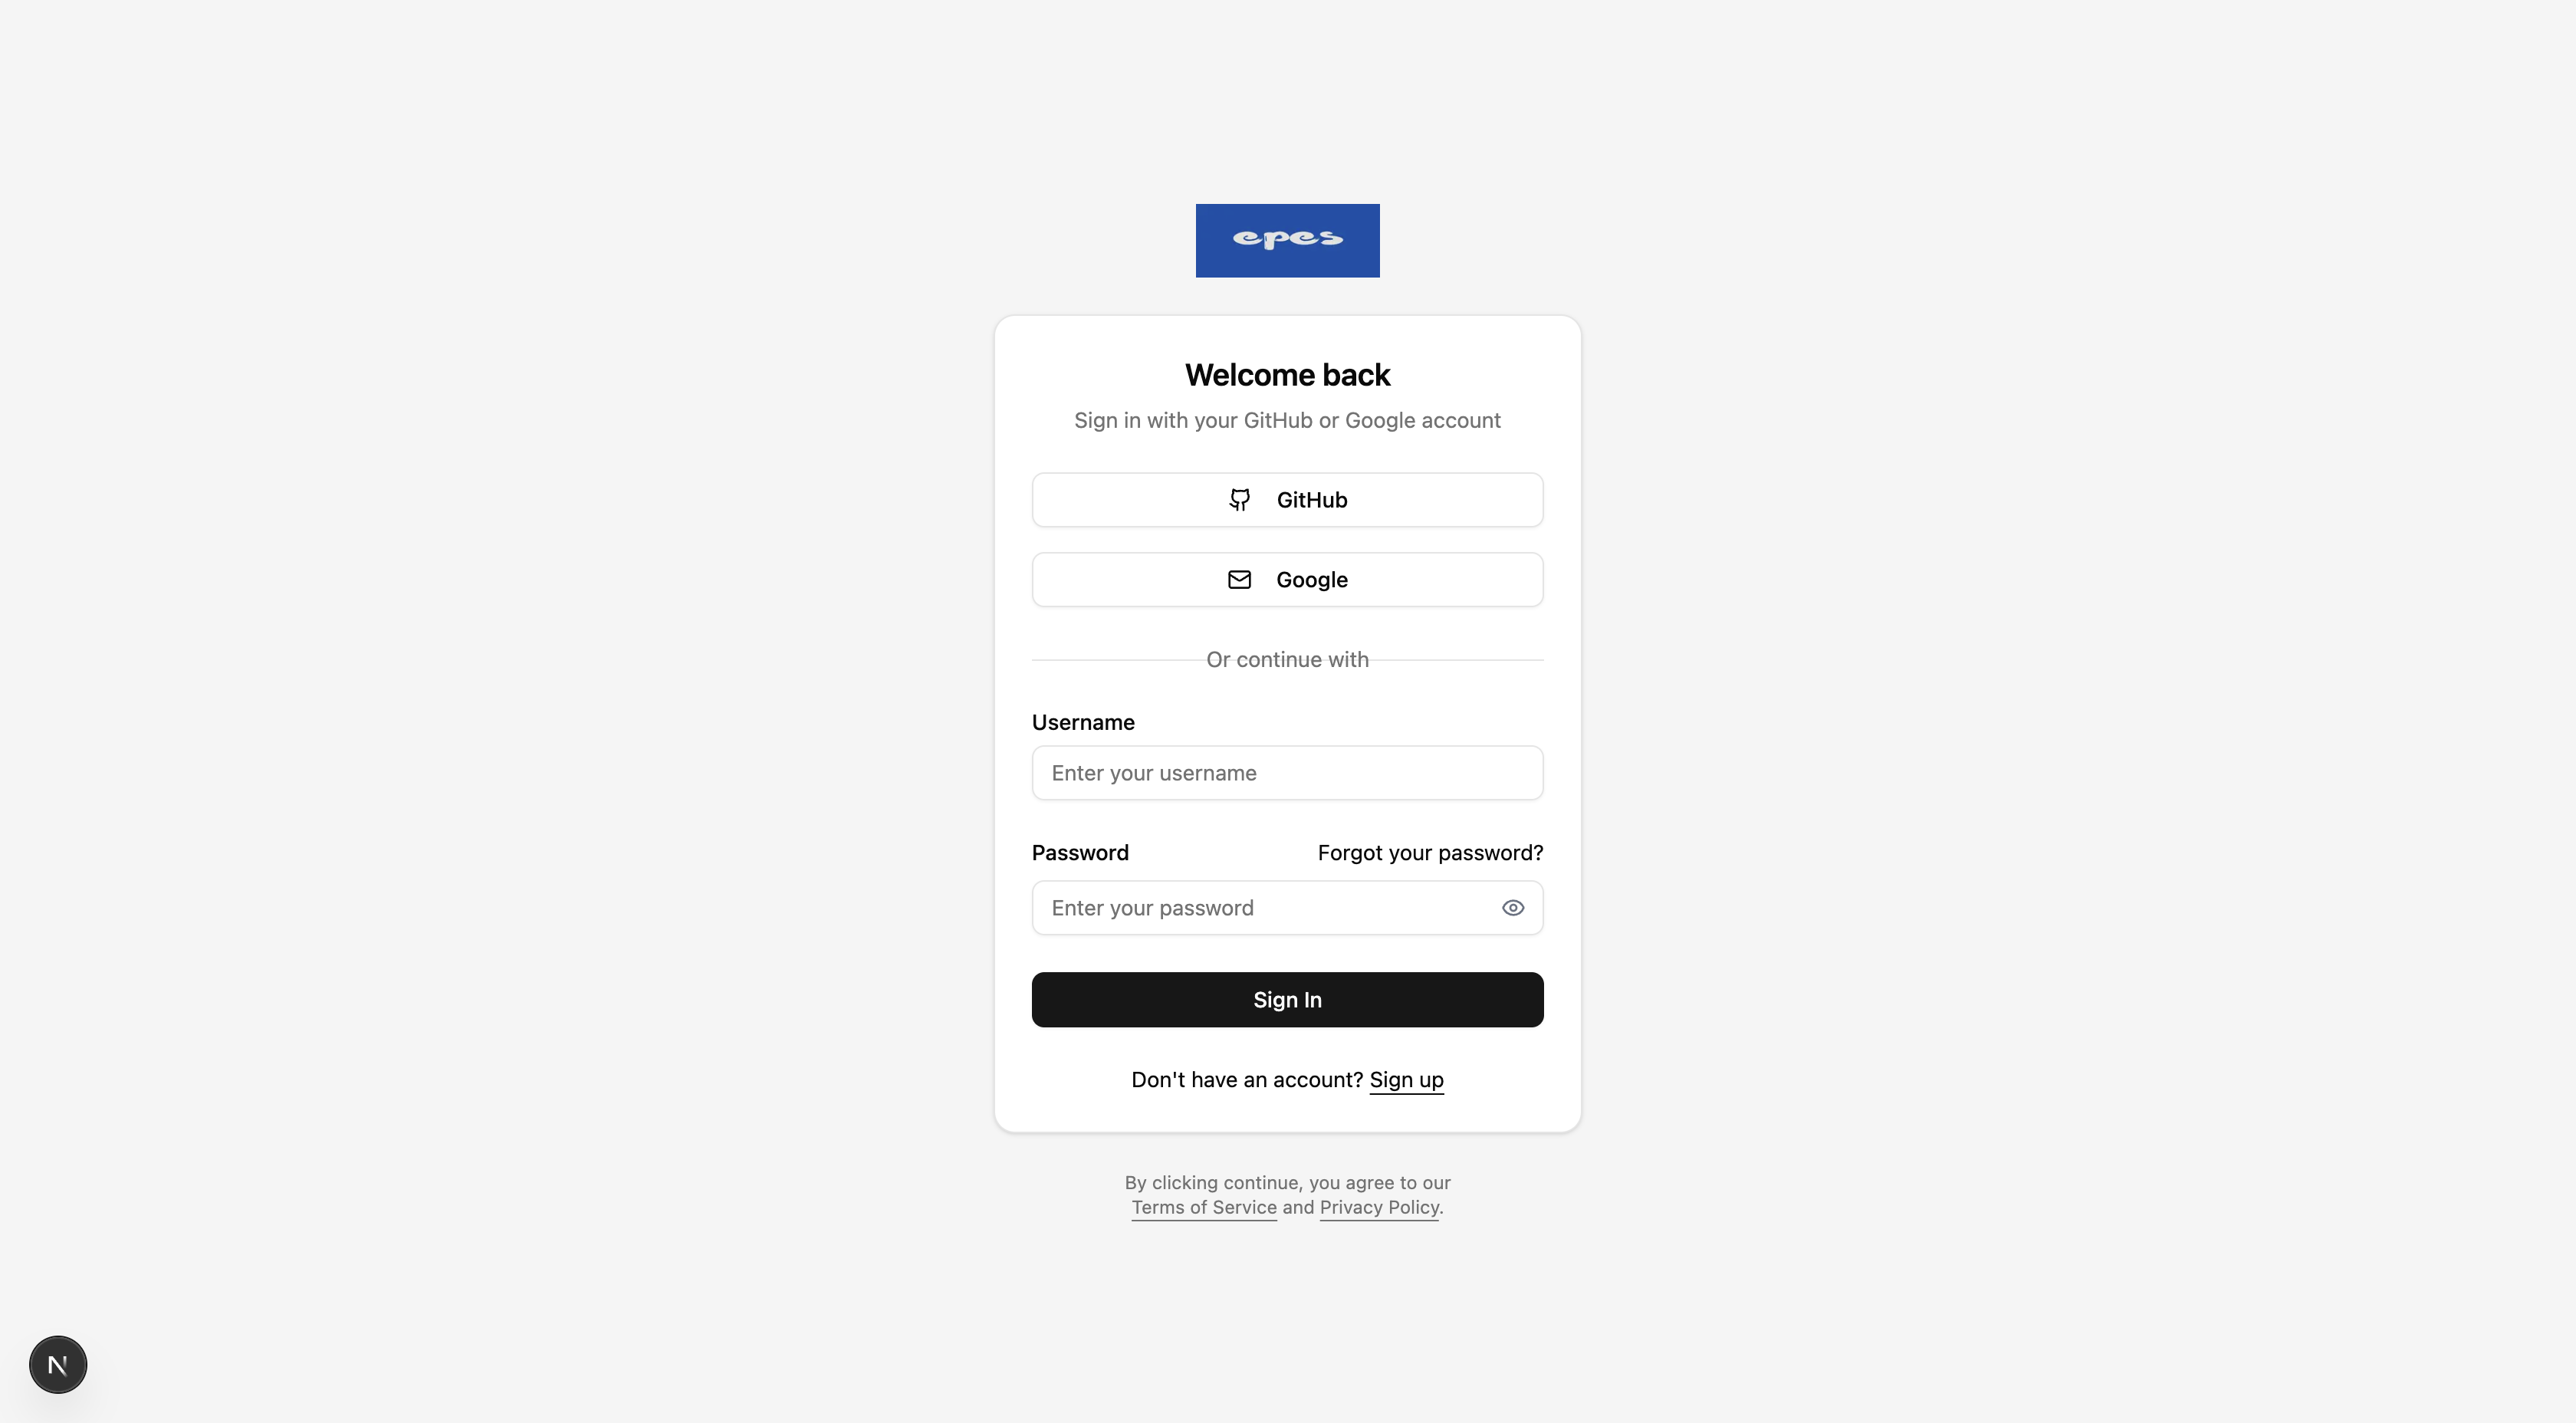
\includegraphics[scale=0.3]{src/images/uiux/login.png}
    \caption{Нэвтрэх хуудас}
    \label{fig:login_page}
\end{figure}

\subsubsection{Системийн ерөнхий хуудаснууд}

\begin{figure}[H]
    \centering
    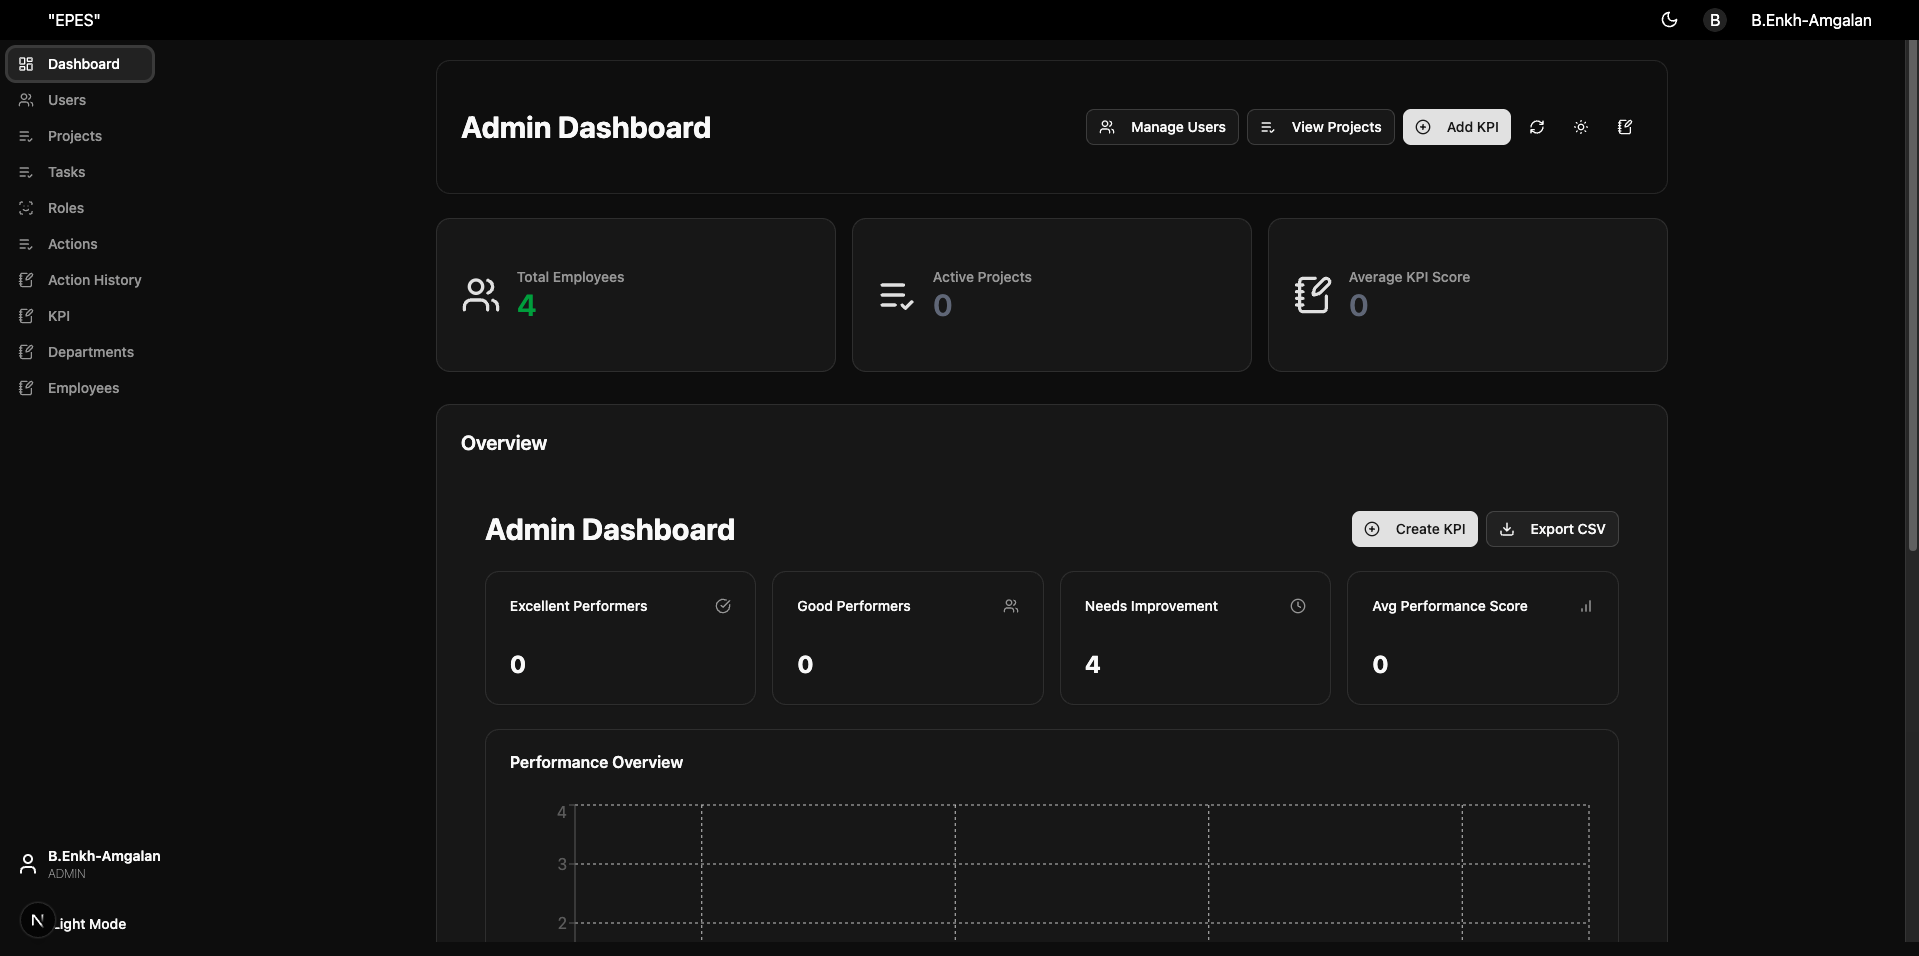
\includegraphics[scale=0.3]{src/images/uiux/adminDash.png}
    \caption{Админ дашбоард харагдац}
    \label{fig:admin_dashboard_page}
\end{figure}

\begin{figure}[H]
    \centering
    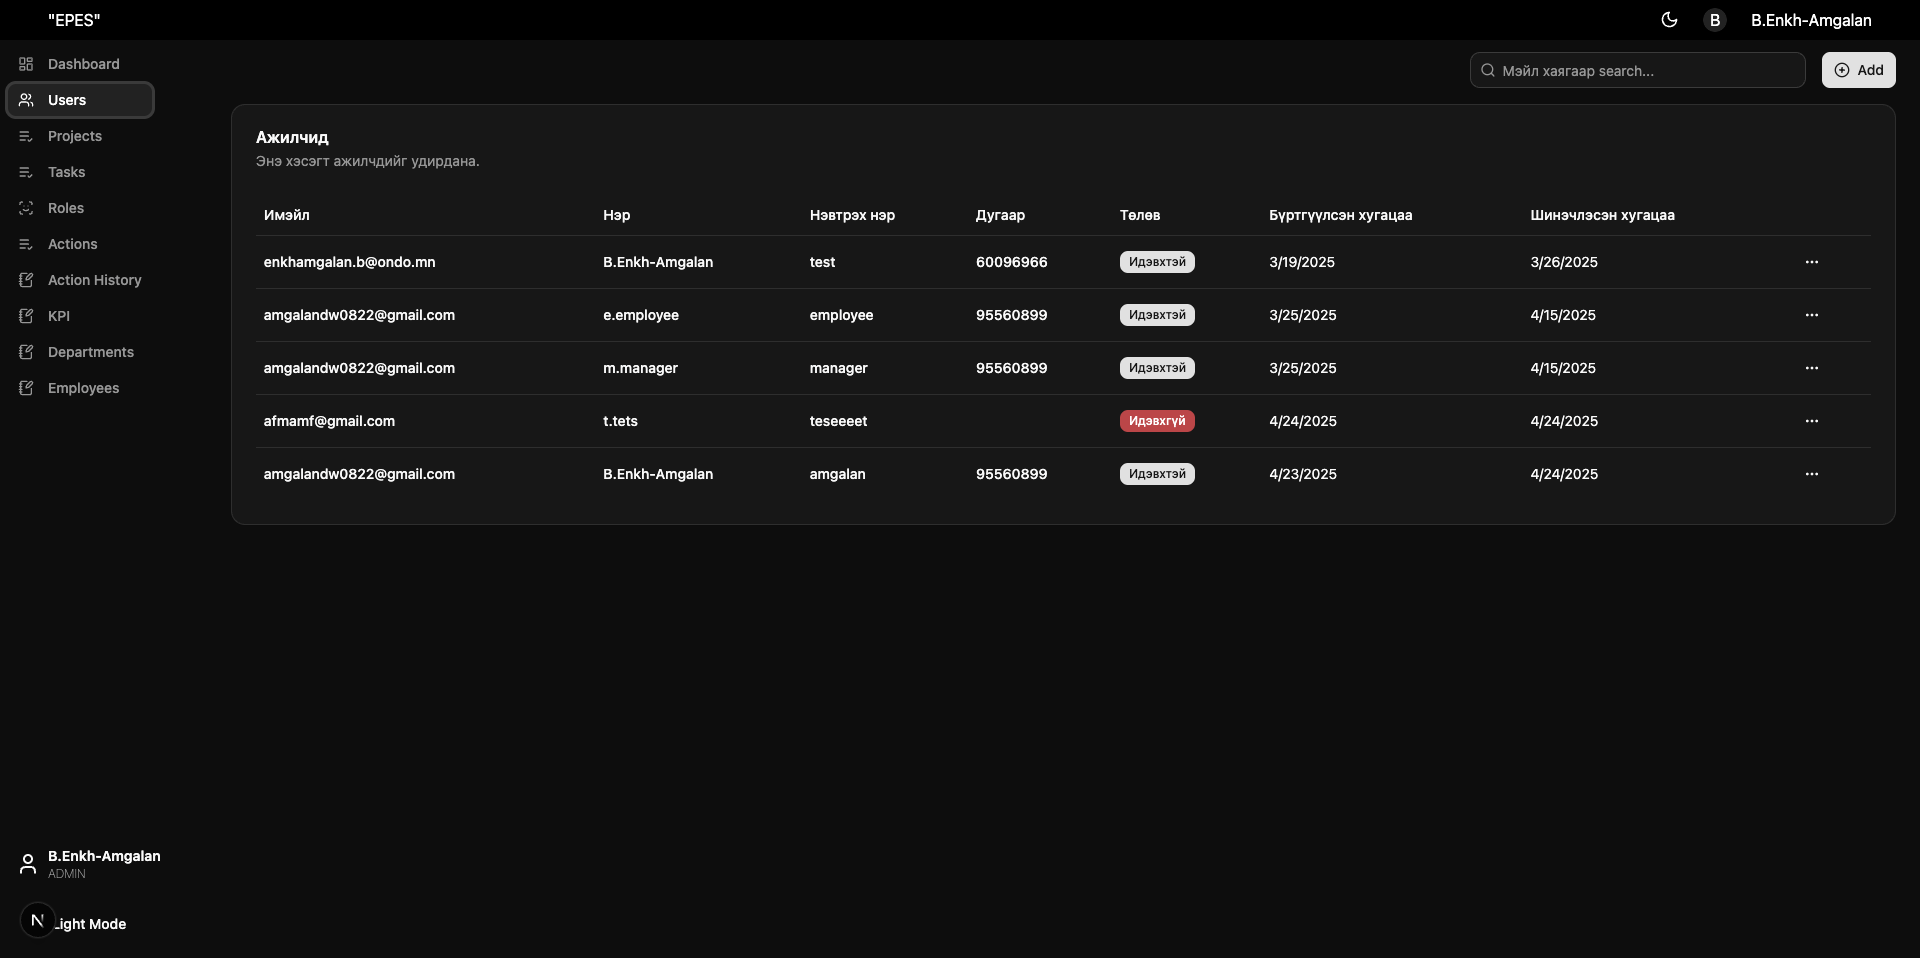
\includegraphics[scale=0.3]{src/images/uiux/listEmp.png}
    \caption{Ажилтны жагсаалт}
    \label{fig:list_emp_page}
\end{figure}

\begin{figure}[H]
    \centering
    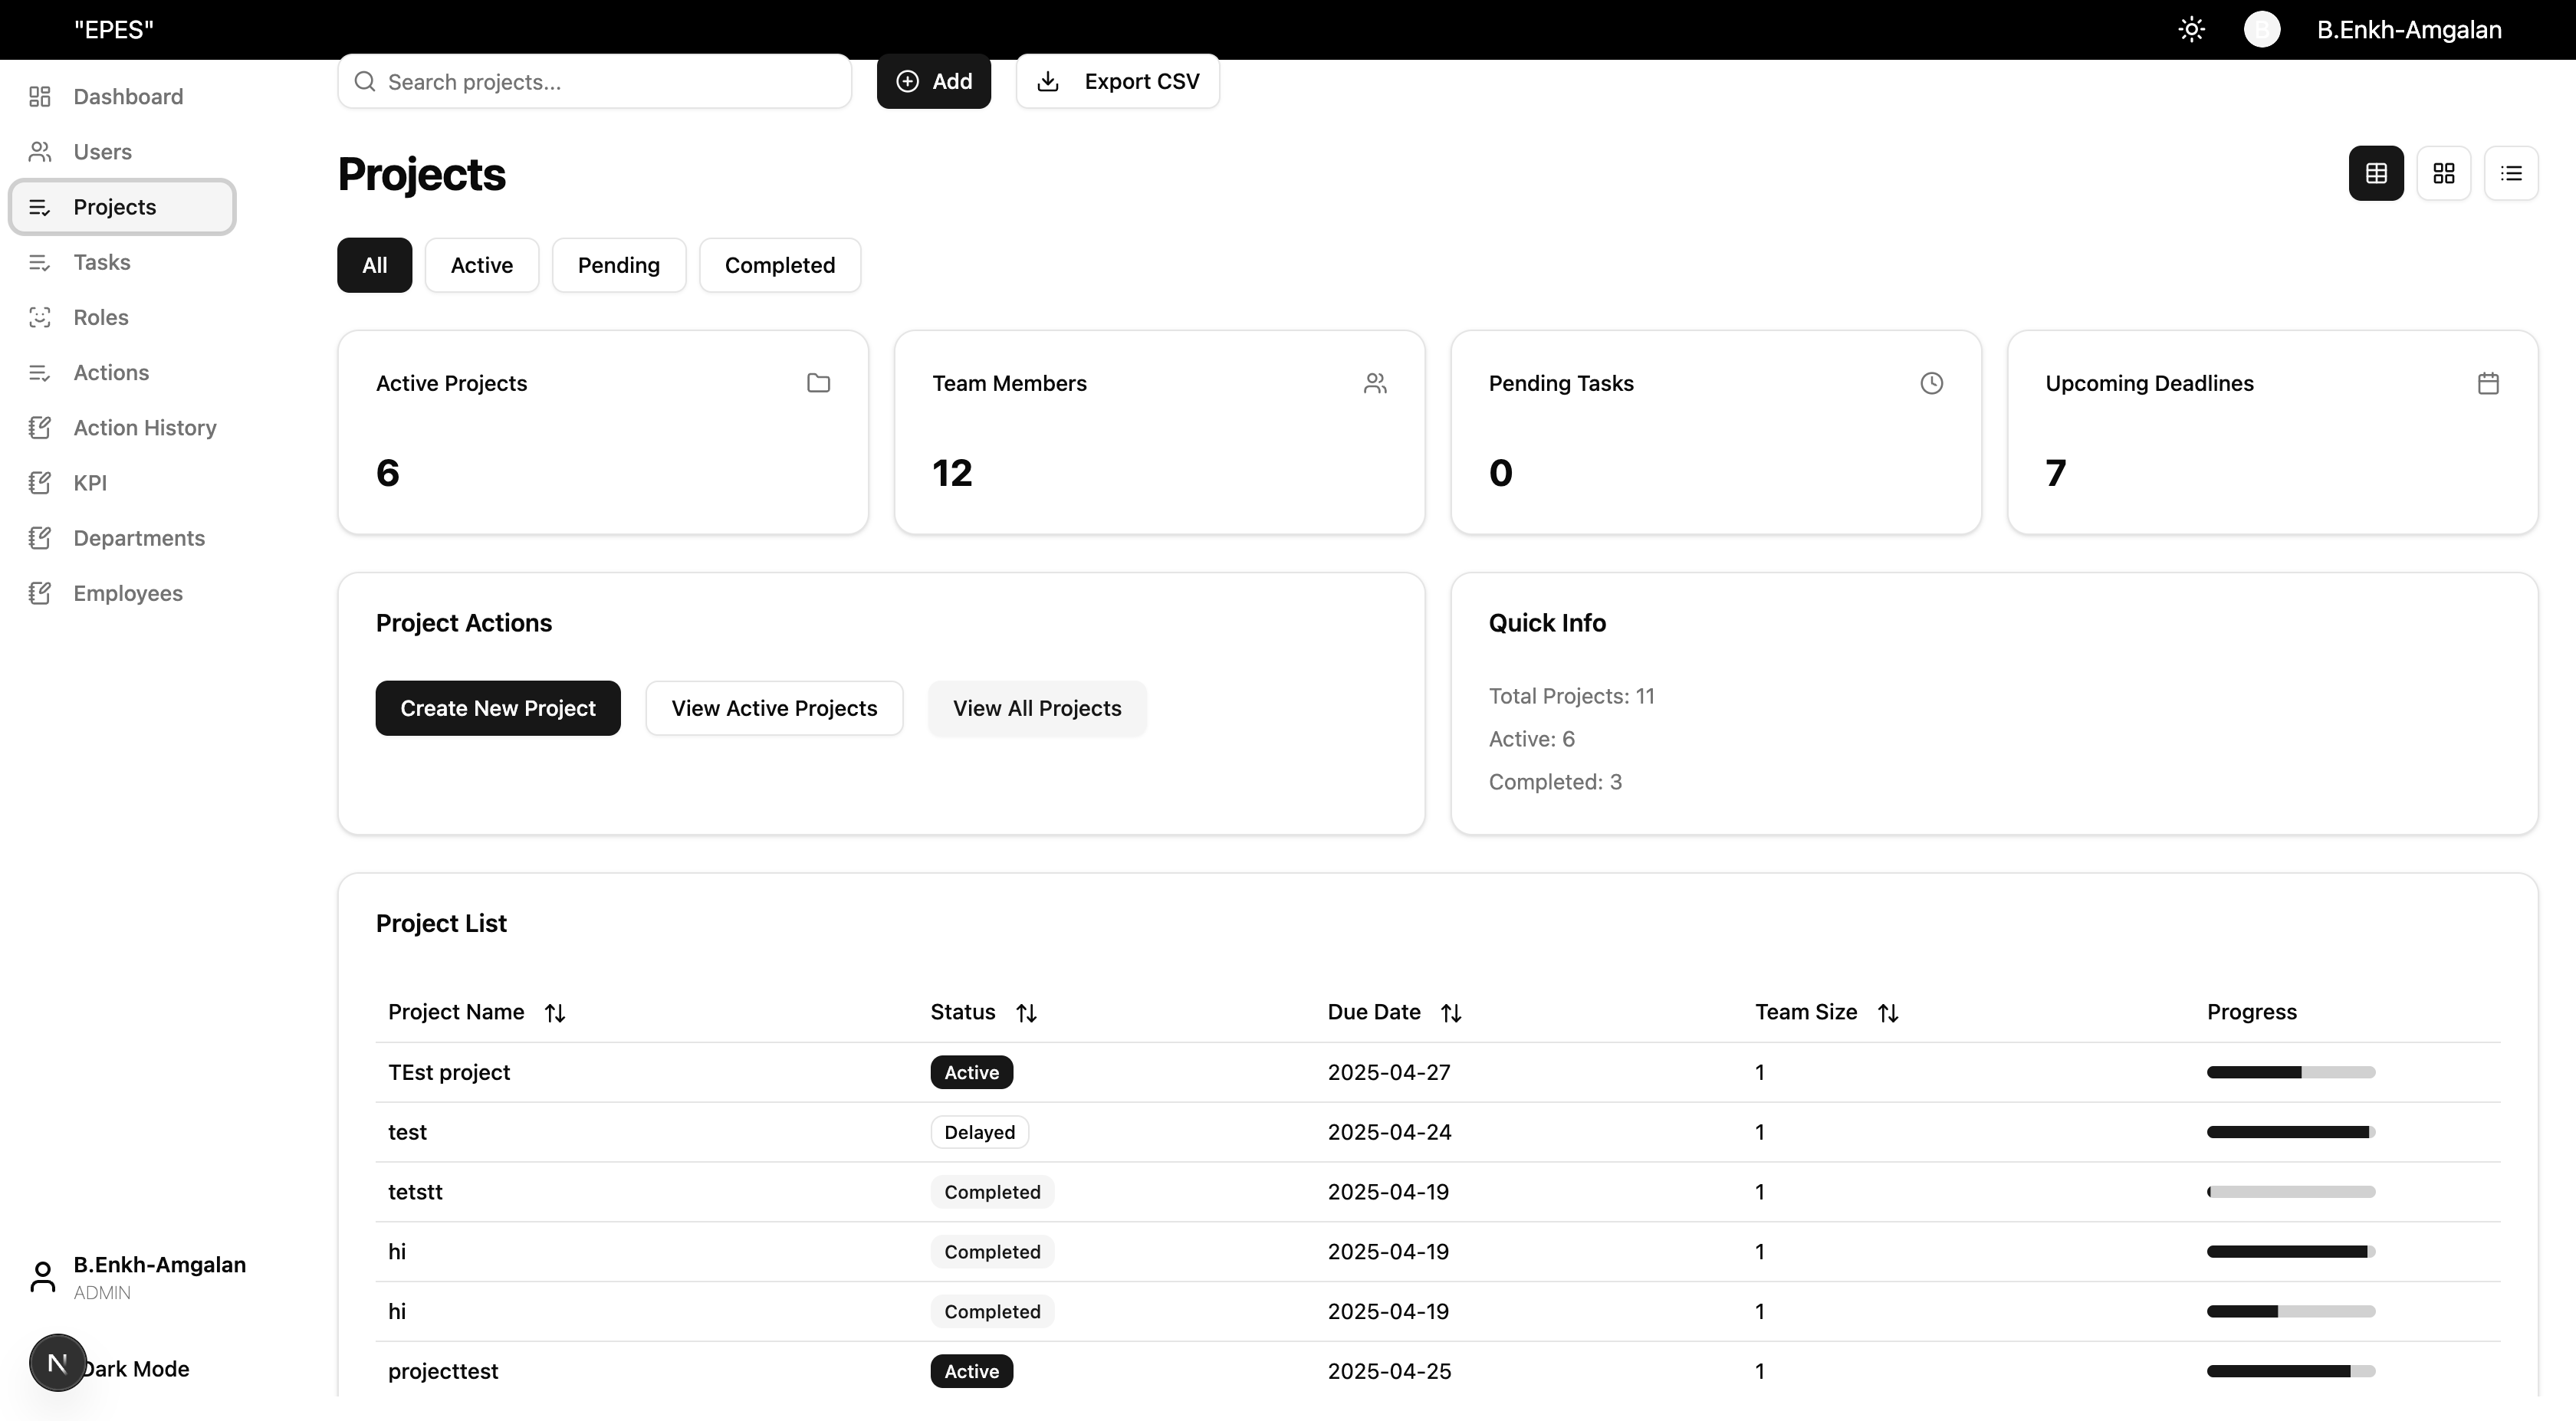
\includegraphics[scale=0.3]{src/images/uiux/proj.png}
    \caption{Төслийн харагдац}
    \label{fig:proj_page}
\end{figure}

\begin{figure}[H]
    \centering
    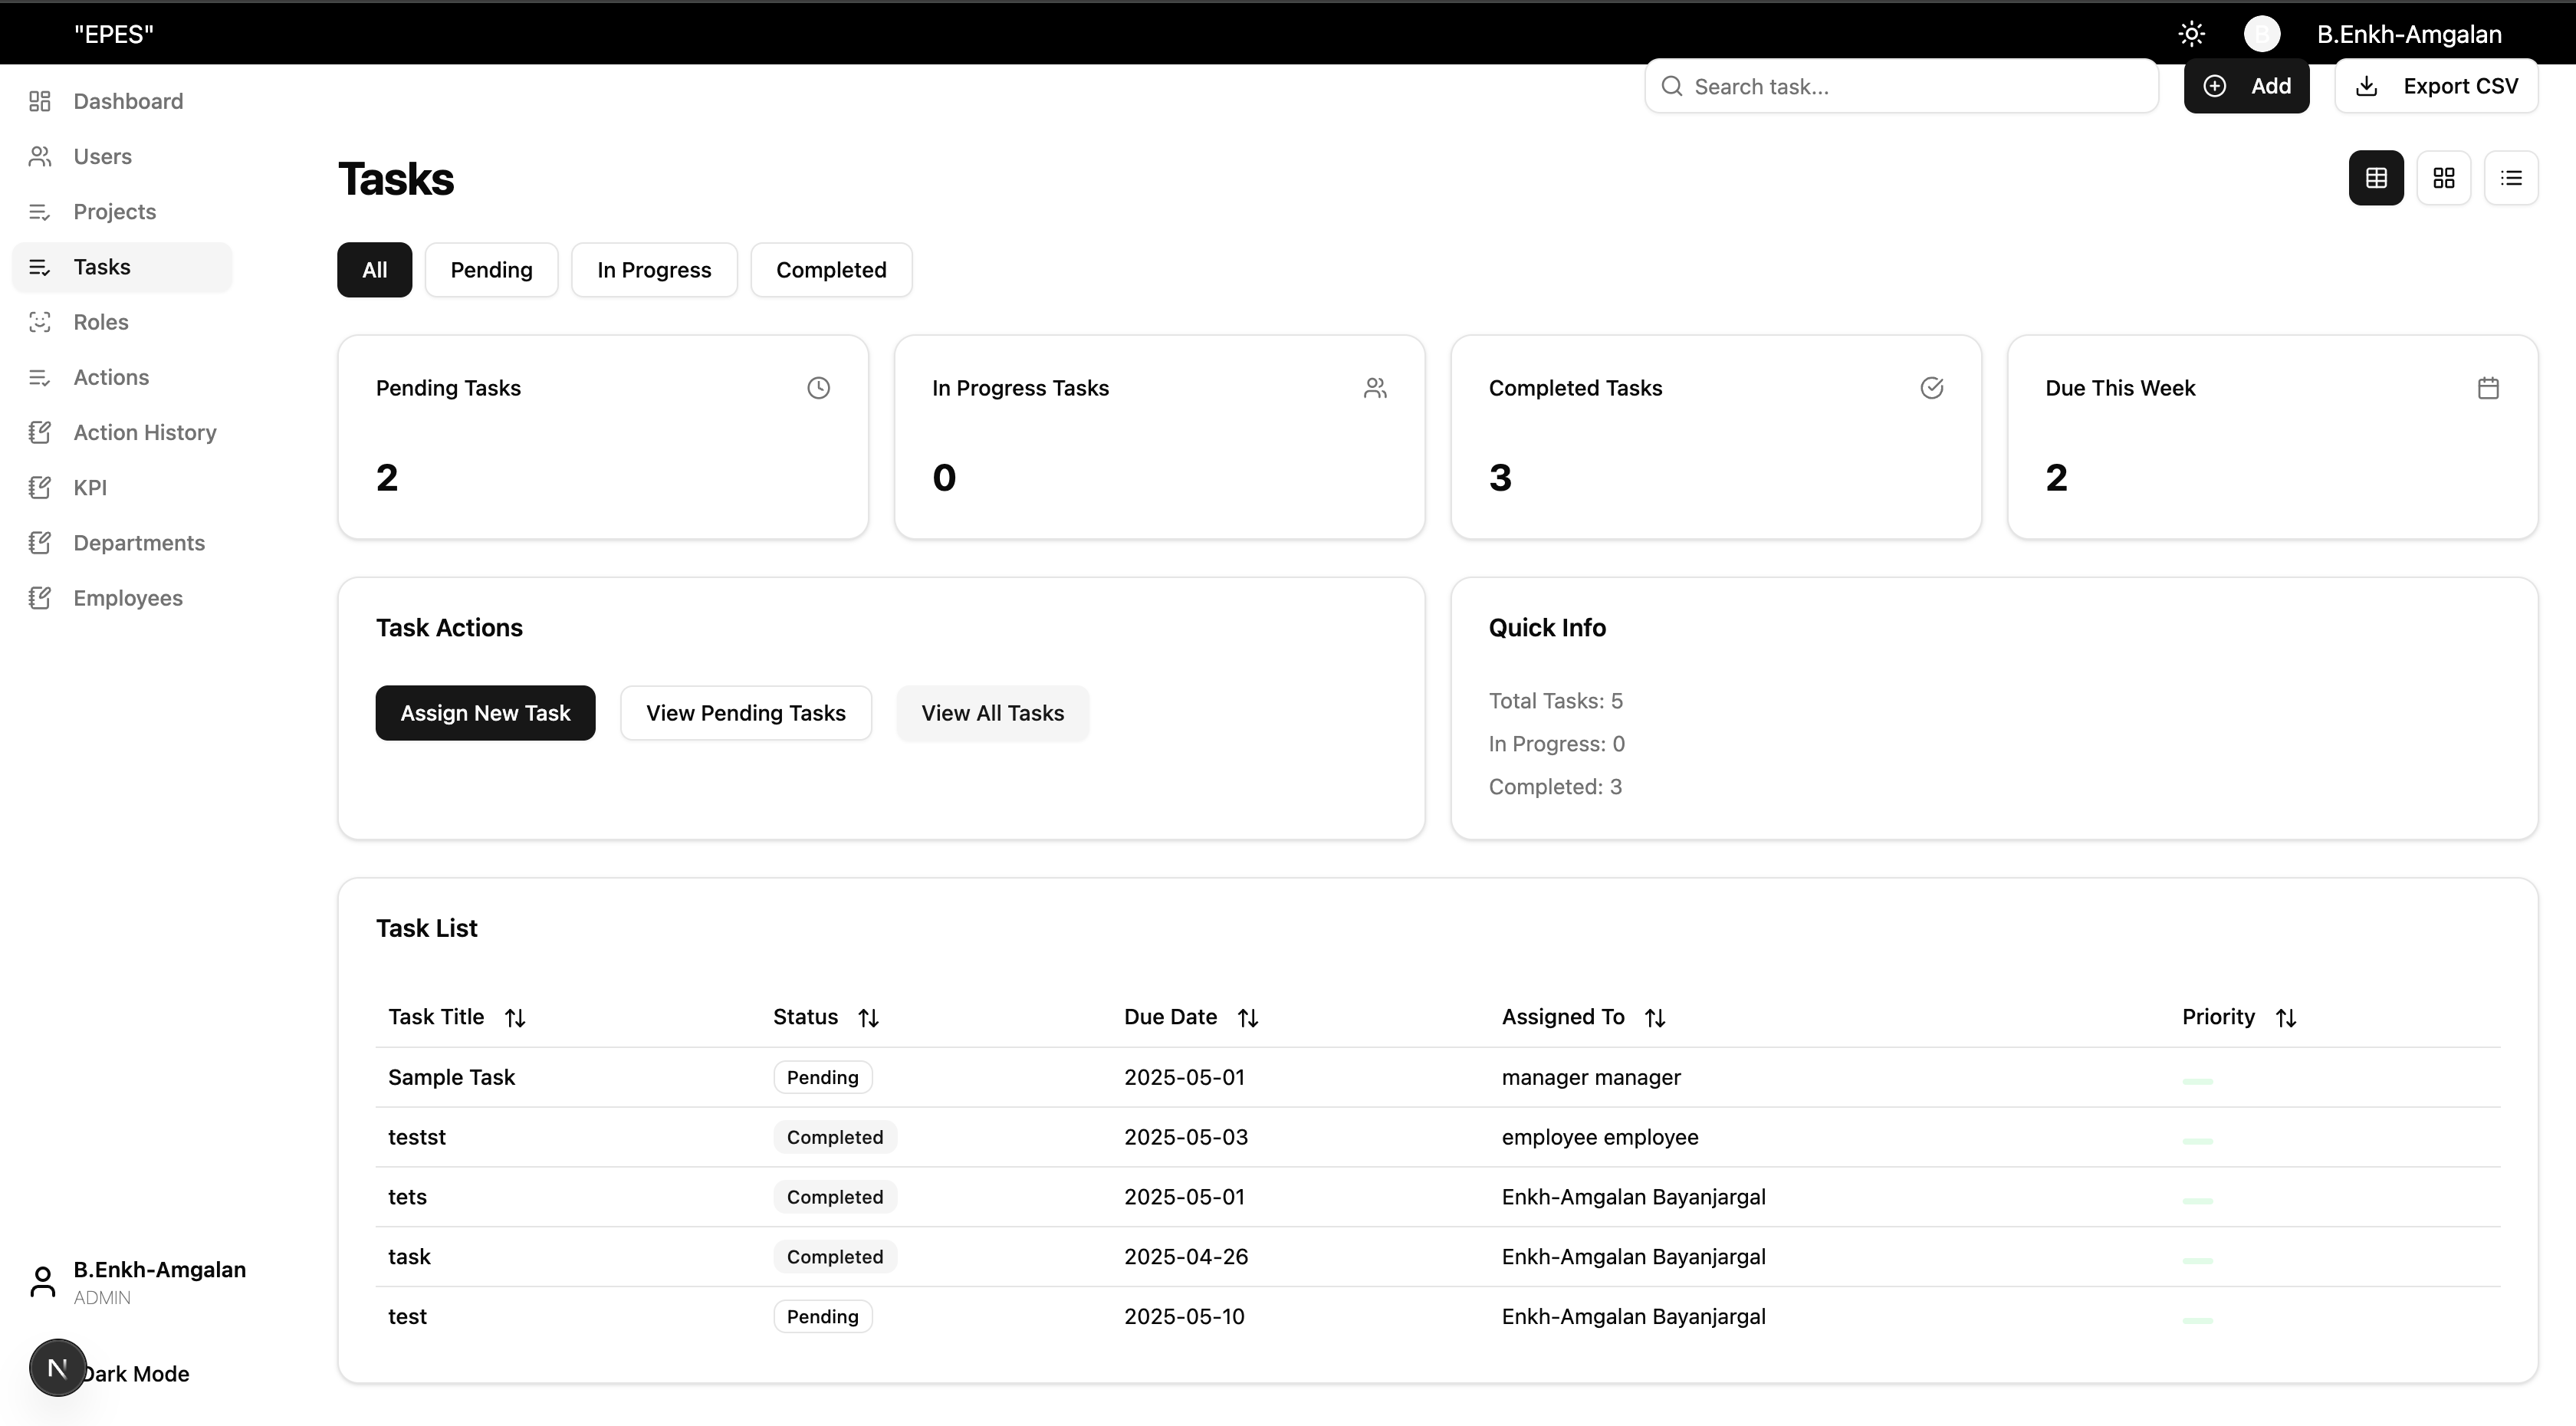
\includegraphics[scale=0.3]{src/images/uiux/task.png}
    \caption{Даалгаварын харагдац}
    \label{fig:task_page}
\end{figure}

\begin{figure}[H]
    \centering
    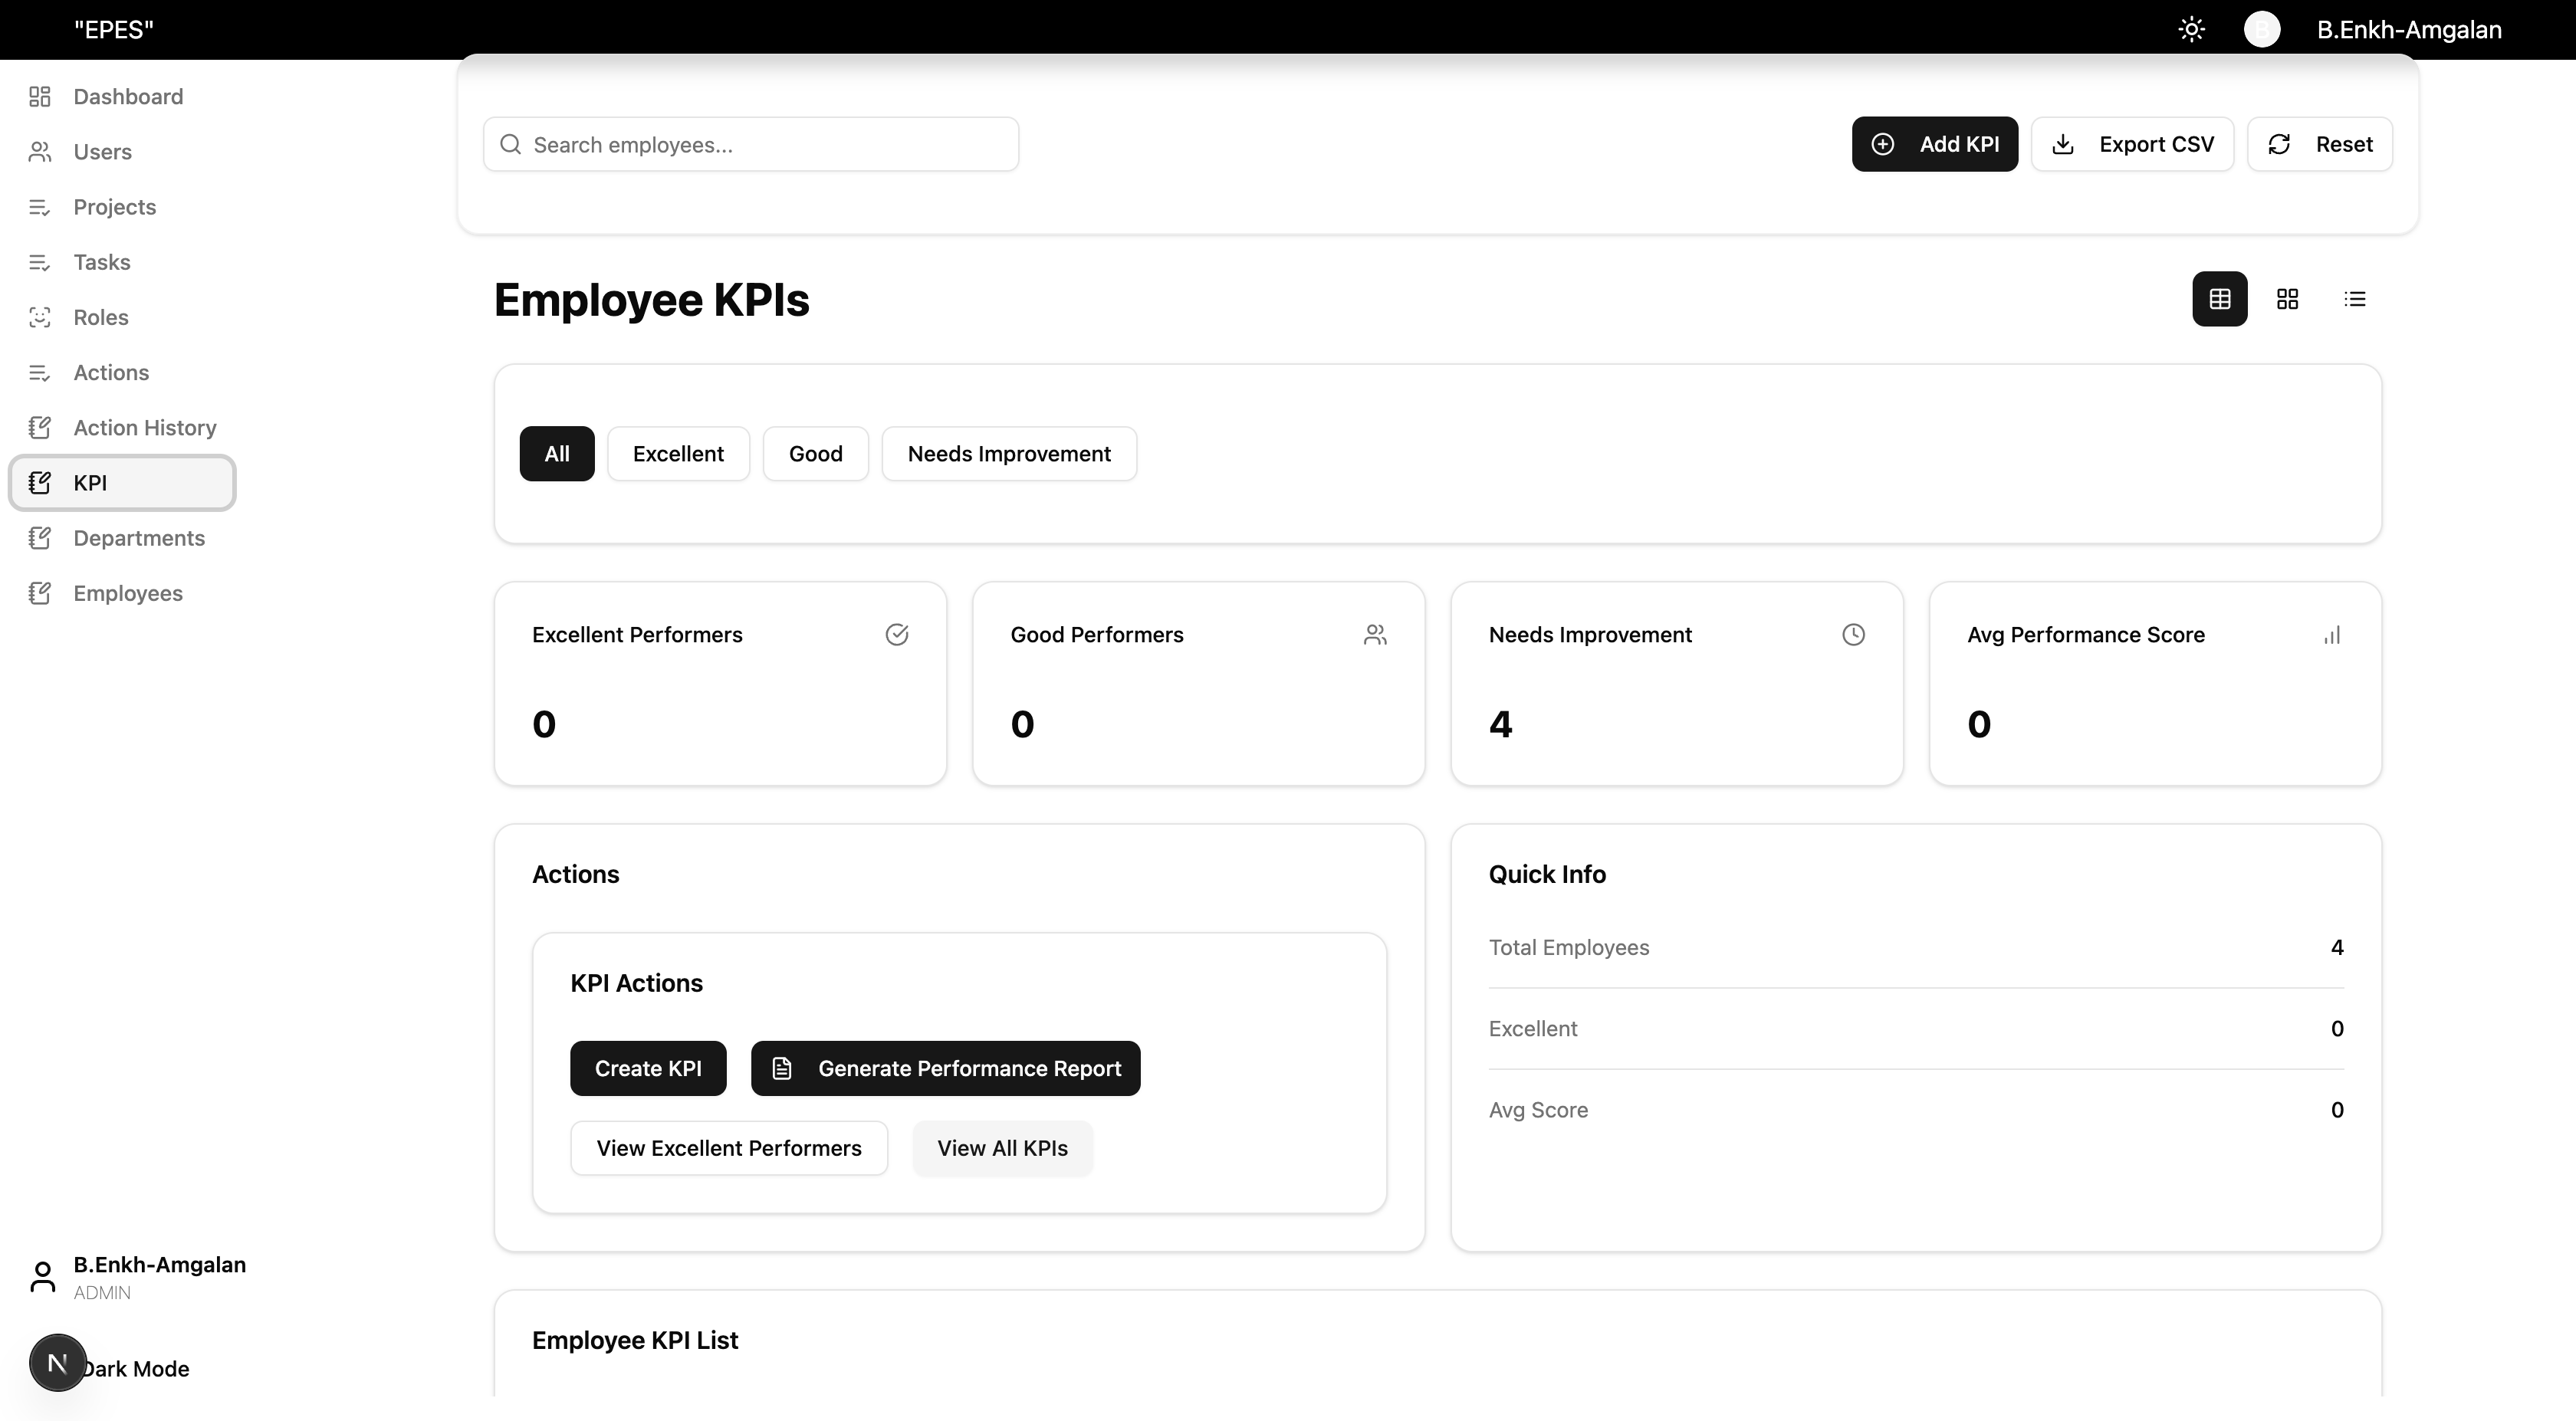
\includegraphics[scale=0.3]{src/images/uiux/kpi.png}
    \caption{Гүйцэтгэлийн үнэлгээний харагдац}
    \label{fig:kpi_page}
\end{figure}

\begin{figure}[H]
    \centering
    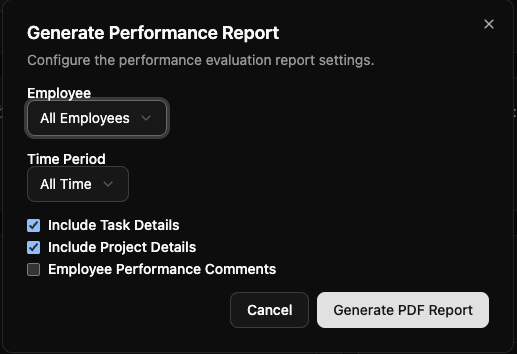
\includegraphics[scale=0.8]{src/images/uiux/reportgen.png}
    \caption{Тайлан гаргах компонентийн харагдац}
    \label{fig:report_gen_comp}
\end{figure}

\begin{figure}[H]
    \centering
    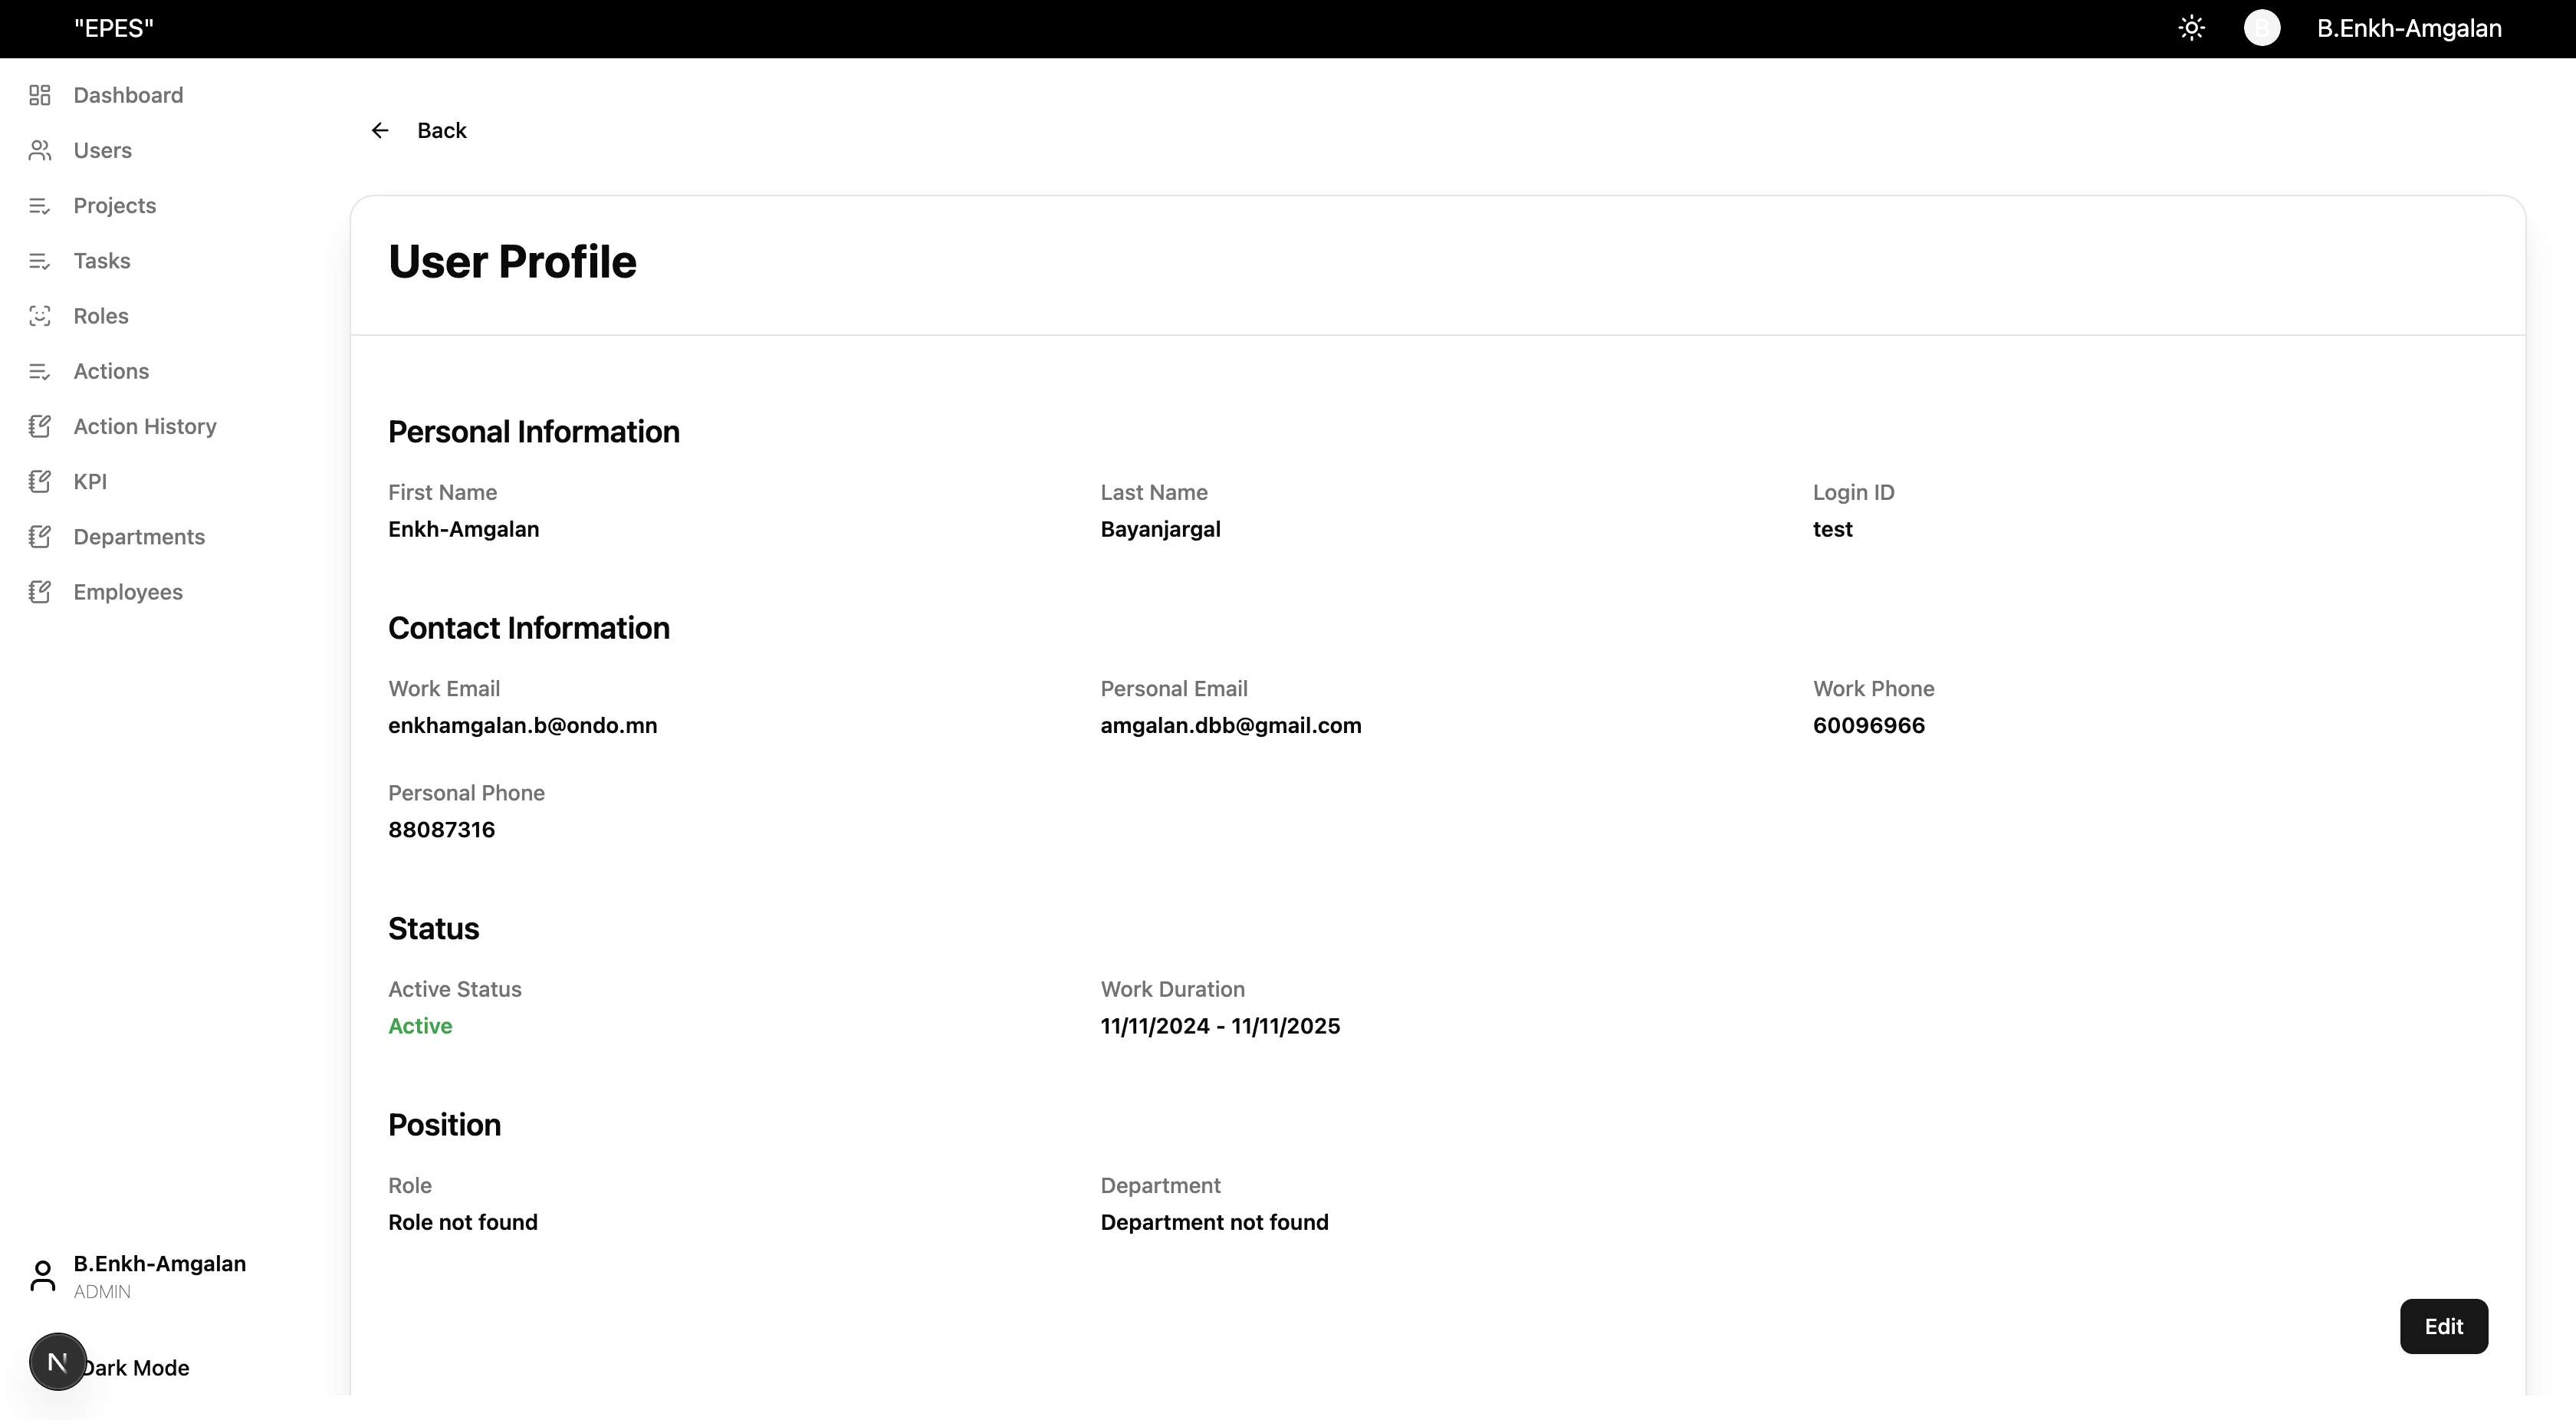
\includegraphics[scale=0.3]{src/images/uiux/userProfile.png}
    \caption{Хэрэглэгчийн профайлын харагдац}
    \label{fig:user_profile_page}
\end{figure}
\pagebreak